\documentclass[a4paper, 10pt]{article}
\usepackage[a4paper, total={6in, 10in}]{geometry}
\usepackage[printsolution=false]{exercises}
\usepackage{url}
\usepackage{background, hyperref}
\usepackage{tcolorbox}
\usepackage{lastpage}
\usepackage{fancyhdr}
\usepackage{xcolor}
\usepackage[sfdefault]{cabin}
\usepackage{graphicx}
\usepackage{wrapfig}
\usepackage[T1]{fontenc}
\usepackage[backend=bibtex,style=authoryear,natbib=true, maxbibnames=9, maxcitenames=2]{biblatex}
\bibliography{howeetal18.bib}
\usepackage{todonotes}
%\bibliographystyle{besjournals}
\setlength\parindent{0pt}
\pagestyle{fancy}
\fancyhead[L,C,R]{}
\fancyfoot[L]{\small CTDS workshop, Univ. of St Andrews}
\fancyfoot[R]{\small Practical 2 - duiker detections}
\fancyfoot[C]{\small \thepage\ of \pageref{LastPage}}
\renewcommand{\headrulewidth}{0pt}
\renewcommand{\footrulewidth}{1pt}

\newif\iffirstpage
\firstpagetrue
\backgroundsetup{contents={%
 			\iffirstpage
				\includegraphics[width=\textwidth]{jaguar1.jpg}%
				\global\firstpagefalse
				\fi
			},
			scale=1,placement=top,opacity=0.6,position=current page.north, vshift=-1cm
}

\begin{document}
%% don't mess with blank lines here in the title.
\phantom{a}

\vspace{4.7cm}

{\Large Camera trap distance sampling workshop}

{\large 21-25 March 2022}

\begin{flushright}
\tiny{Source: \url{https://unsplash.com/@satyadeep_d}}
\end{flushright}

\ifsolutionthenelse{%
{\Large \color{blue}Solution \\}
{\color{blue}\rule{\linewidth}{0.5mm}}
}%
{%
}

A distance sampling approach to the analysis of camera trapping data offers the potential advantage that individual animal identification is not required. However, accurate animal-to-camera detection distances are required. This requires calibration prior to the survey with images of objects of known size taken at known distances from the camera. See details in \citep{howeetal} for description of the field work and data analysis. Here we present analysis of data from \citep{howeetal} using Distance for Windows \citep{Thomas2010}. 

\section{Data input}

A data set for recording of detections during daytime are in the Distance for Windows project associated with this practical.  The data themselves are in an online repository \citep{dryad}

\begin{tcolorbox}[colback=yellow!5!white, colframe=yellow!60!black, title=Access duiker project]
Open the DistWin project \texttt{DuikerDaytime} found in the Sample Projects folder.  This project was installed when you installed the DistWin software.  We will make some modifications to the basic project.
\end{tcolorbox}

Glance through the data window, noting one camera station (E4) had no detections.  Also inspect the field included in the Global layer labelled \emph{Sampling fraction}.  This is the proportion of the full field of view that the camera can "see" ($42^\circ$; 42/360=0.11667). We will address the other fields in the Global layer in a later practical.

\begin{wrapfigure}{r}{0.35\textwidth}
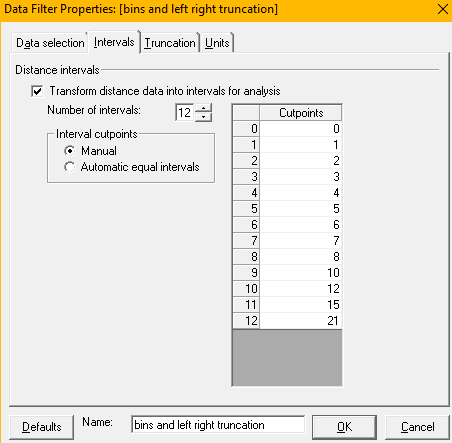
\includegraphics[width=0.33\textwidth]{images/bins-datafilter.png}
\caption{Specifying the cutpoints for the distance bins. \label{fig:bins}}
\vspace{-25pt}
\end{wrapfigure}

\subsection{Distance recording: binning and truncation}

Distance bins are set to be narrow out to 8m, then increasing in width to the maximum detection distance of 21m as shown in the Intervals tab of the Data Filter (Fig. \ref{fig:bins})

Data will also be altered for consistency with \citep{howeetal} by invoking truncation both at very small distances and at large distances.

As described in \citet{howeetal}
\begin{quotation}
a paucity of observations between 1 and 2 m but not between 2 and 3 m, so we left-truncated at 2 m. Fitted detection functions and probability density functions were heavy-tailed when distances >15 m were included, so we right truncated at 15 m.
\end{quotation}

Note that because the data have been binned, the left and right truncation distances can only be selected from the binning cutpoints (Fig. \ref{fig:truncation}).

\begin{wrapfigure}{r}{0.35\textwidth}
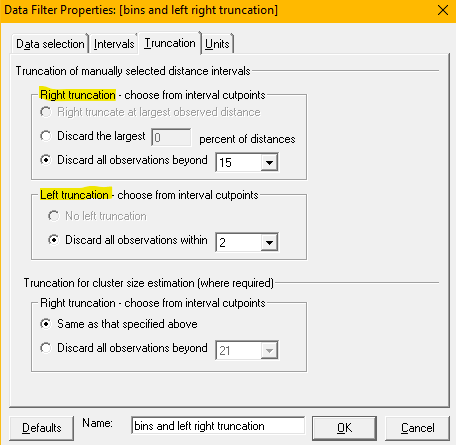
\includegraphics[width=0.33\textwidth]{images/truncation-datafilter.png}
\caption{The \emph{Data Filter} defining left and right truncation. \label{fig:truncation}}
\vspace{-25pt}
\end{wrapfigure}

\section{Detection function modelling}

Before constructing any detection function models, we will organise our project suited to our needs for this practical: create an analysis set and alter the \emph{Results Browser}.

\subsection{Create a new analysis set}
\begin{wrapfigure}{r}{0.35\textwidth}
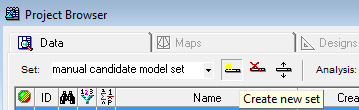
\includegraphics[width=0.33\textwidth]{images/new-set.png}
\caption{Create a new analysis set. \label{fig:newset}}
\vspace{-25pt}
\end{wrapfigure}


So as not to mingle the analyses you will be performing with analyses present in the Sample Project, create a new analysis set.  This is accomplished by pressing the \emph{New Set} button  (Fig. \ref{fig:newset}).  Give it a memorable name, e.g. \emph{detection function models}.  This analysis set will store all of the candidate models described below.
%\vspace{3cm}

\subsection{Adjust columns of \emph{Results Browser}}

For detection function model fitting, we need only have the following statistics in the \emph{Results Browser}
\begin{itemize}
	\item number of model parameters
	\begin{itemize}
		\item total
		\item key function parameters
		\item adjustment term parameters
	\end{itemize}
	\item Delta AIC
	\item AIC
	\item P-value of $\chi^2$ goodness of fit test
	\item probability of detection $P$
	\item $CV(P)$
\end{itemize} 

These statistics can be selected from the list of available statistics using the \emph{Column browser} (Fig. \ref{fig:columns}).

\begin{wrapfigure}{l}{0.35\textwidth}
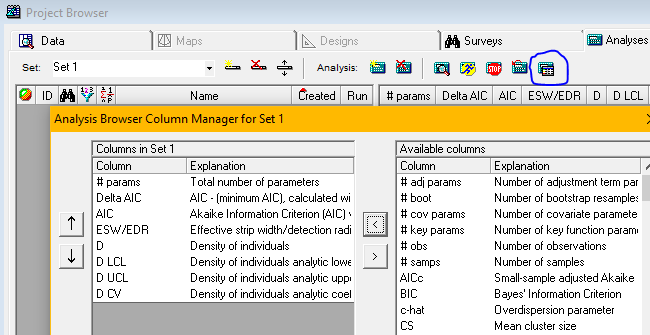
\includegraphics[width=0.33\textwidth]{images/column-mgr.png}
\caption{Select statistics to appear in \emph{Results Browser}. \label{fig:columns}}
\vspace{-25pt}
\end{wrapfigure}

\subsection{Model construction and fitting}
Following the adjustments to the data and organising your Distance for Windows project, creation of detection function models begins.  Specify the set of models to be fitted to the binned and truncated data.  We restrict our candidate models to those with three or fewer parameters and we only consider one type of adjustment for each of the key functions.  These criteria lead to a slightly different set of candidate models than that used in \citet{howeetal}.

Candidate models include 
\begin{itemize}
	\item uniform key with 1, 2 and 3 cosine adjustments, 
	\item half normal key with 0, 1 and 2 cosine adjustments and
	\item hazard rate key with 0 and 1 simple polynomial adjustments. 
\end{itemize}
 
 Note, rather than allow Distance for Windows to perform within-key function model selection of adjustment terms, we explicitly fit each adjustment term model. To convince Distance for Windows to fit a model with a fixed number of adjustment terms, we manually choose the number of adjustment terms for the model being specified (shown in Fig. \ref{fig:manual}).
 
\begin{wrapfigure}{l}{0.35\textwidth}
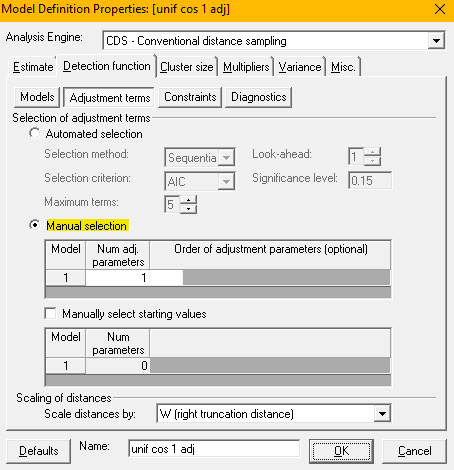
\includegraphics[width=0.33\textwidth]{images/manual-adjterms.png}
\caption{Manual specification of the number of adjustment terms. \label{fig:manual}}
\vspace{-35pt}
\end{wrapfigure} 

We are not yet interested in estimates of duiker density, that field is not visible in our Results Browser.  Therefore the effect of multipliers is not visible at this stage of the analysis.  Nevertheless check the \emph{Multipliers} button noting the \emph{Sampling fraction} is incorporated into the analysis.

\section{Model criticism}

Having fitted the eight models described above, use the methods described in Practical 1 to evaluate the fitted models. If any models return an amber (warning) or red (error) status light, understand the reason(s) for the warnings or errors. 

Elements of this assessment should include goodness of fit (with binned data, the $\chi^2$ test is the only test available) and the AIC metrics both found in the \emph{Results Browser}.  

At the moment, we are not interested in the density estimates produced by these analyses, because there are additional elements yet to be incorporated.  We have removed the density estimates from the \emph{Results Browser} for this phase of the analysis.

\ifsolutionthenelse{%
	\begin{tcolorbox}[colback=green!5!white, colframe=green!60!black, title=Results browser for fitted models]
{\small
\begin{tabular}{lrrrrrrrr}
Name                 & Par & Key par & Adj par & $\Delta$AIC & AIC     & GOF Chi-p & P     & CV(P) \\
\hline
uniform cosine 1adj  & 1        & 0            & 1            & 80.3      & 44092.5 & 0.000     & 0.300 & 0.005 \\
uniform cosine 2adj  & 2        & 0            & 2            & 74.6      & 44086.8 & 0.000     & 0.284 & 0.019 \\
uniform cosine 3adj  & 3        & 0            & 3            & 0.0       & 44012.2 & 0.000     & 0.329 & 0.039 \\
halfnorm cosine 0adj & 1        & 1            & 0            & 133.0     & 44145.2 & 0.000     & 0.257 & 0.012 \\
halfnorm cosine 1adj & 2        & 1            & 1            & 20.4      & 44032.6 & 0.000     & 0.326 & 0.037 \\
halfnorm cosine 2adj & 3        & 1            & 2            & 19.4      & 44031.6 & 0.000     & 0.334 & 0.060 \\
hazard simple 0adj   & 2        & 2            & 0            & 20.5      & 44032.7 & 0.000     & 0.375 & 0.012 \\
hazard simple 1adj   & 3        & 2            & 1            & 9.6       & 44021.8 & 0.000     & 0.366 & 0.015
\end{tabular}
}
\end{tcolorbox}
}
{
}

\section{Questions about this analysis}

\begin{itemize}
\item What might be justification for left truncation?
\ifsolutionthenelse{%
	\begin{tcolorbox}[colback=green!5!white, colframe=green!60!black, title=Left truncation]
	If animals close to the detector respond, detections (or lack thereof) may not be representative of the detection process. Similarly, if the vertical field of view of the detectors do not detect animals short in stature close to the detector, then left truncation might be justified. 
\end{tcolorbox}
}
{
}
	\begin{itemize}
		\item What are the dangers of such truncation?
\ifsolutionthenelse{%
	\begin{tcolorbox}[colback=green!5!white, colframe=green!60!black, title=Left truncation challenges]
		The truncation distance is subjective.  Remember it is detections at small distances that are fundamental to estimating $\hat{h}(0)$: slope of the PDF at distance 0.  This estimate is estimated via extrapolation when left truncation is used.
		\end{tcolorbox}
}
{
}
	\end{itemize}
\item Initial assessment of fit of models?
\ifsolutionthenelse{%
	\begin{tcolorbox}[colback=green!5!white, colframe=green!60!black, title=Model fit]
Note the P-values for all goodness of fit tests are effectively zero, meaning none of the models fit the data because of overdispersion.
		\end{tcolorbox}
}
{
}
\item What is your preliminary model choice?
\ifsolutionthenelse{%
	\begin{tcolorbox}[colback=green!5!white, colframe=green!60!black, title=Model selection]
Using traditional AIC for model selection, we conclude the uniform key function with 3 cosine adjustments is the preferred model of the eight models fitted.  This differs from the analysis reported in \citep{howeetal} because the uniform key with three cosine adjustments was not included in the candidate model set those authors fitted to these data.
		\end{tcolorbox}
}
{
}\end{itemize}

\printbibliography

\end{document}